\subsection*{Модель композиции приложения в COCOMO II}

\subsection*{Описание модели}

Для оценки стоимости проекта на ранней стадии конструирования (создание прототипов, макетирование пользовательских интерфейсов, анализ осуществимости, оценка производительности, определение степени зрелости технологии) используется модель композиции приложения. Для такой модели характерны грубые входные данные, оценки низкой точности, приблизительные требования и архитектура на уровне концепции.

В качестве единицы измерения используется \textbf{объектная точка} --- средство косвенного измерения программного обеспечения. Определение числа
объектных точек производится с учетом количества экранов (как элементов
пользовательского интерфейса), отчетов и компонентов, требуемых для построения приложения, в соответствии со следующими правилами:

\begin{itemize}
    \item[---] простые экранные формы принимаются за одну объектную точку,
умеренной сложности — за две объектные точки, сложные — за три
объектные точки;
    \item[---] простые отчеты принимаются за две объектные точки, умеренной
сложности --- за пять объектных точек, сложные --- за восемь объектных
точек;
    \item[---] модули, написанные на языках программирования третьего поколения,
считаются за десять объектных точек.
\end{itemize}

Новые объектные точки NOP определяются по следующей формуле:

$$\text{NOP} = \text{Объектные точки} \cdot \frac{(100 - \%\text{RUSE})}{100},$$

\noindentгде \%$\text{RUSE}$ --- процент повторного использования кода программы.

Трудозатраты вычисляются так:

$$\text{Трудозатраты} = \frac{\text{NOP}}{\text{PROD}},$$

\noindentгде $\text{PROD}$ --- оценка скорости разработки, определяемая из опытности или возможности разработчика или команды или из зрелости или возможности среды разработки.

Время разработки получается в соответствии с формулой:

$$\text{Время} = 3 \cdot \text{Трудозатраты}^{0.33 + 0.2 \cdot (\text{p} - 1.01)},$$

\noindentгде $\text{p}$ --- показатель степени. Значение показателя степени рассчитывается с учетом факторов, влияющих на показатель степени:

$$\text{p} = \frac{(\text{PREC} + \text{FLEX} + \text{RESL} + \text{TEAM} + \text{PMAT})}{100} + 1.01.$$

\subsection*{Применение}

Из макета интерфейса:

\begin{itemize}
    \item[---] для страницы <<Авторизация>>:
        \begin{itemize}
            \item[---] одна форма средней сложности;
        \end{itemize}
    \item[---] для страницы <<Биржевые сводки>>:
        \begin{itemize}
            \item[---] одна сложная форма (таблица биржевых сводок);
            \item[---] одна форма средней сложности (форма ввода);
        \end{itemize}
    \item[---] для страницы <<Заявки>>:
        \begin{itemize}
            \item[---] одна форма средней сложности (таблица заявок);
            \item[---] одна простая форма (кнопки <<Удалить>> и <<Изменить>>);
        \end{itemize}
    \item[---] для страницы <<Новая заявка>>:
        \begin{itemize}
            \item[---] одна форма средней сложности (форма добавления заявки).
        \end{itemize}
\end{itemize}

Итого:

\begin{itemize}
    \item[---] 1 простая форма;
    \item[---] 4 формы средней сложности;
    \item[---] 1 сложная форма.
\end{itemize}


Разработанное приложение состоит из трех компонентов: первый компонент написан
на SQL, второй --- на С\#, а третий --- на Java. Поэтому в проекте два модуля,
написанных на языках третьего поколения (C\# и Java).

Из условия задания:

\begin{itemize}
    \item[---] \%RUSE = 0 \%;
    \item[---] опытность команды --- низкая.
\end{itemize}

\subsubsection{Факторы, влияющие на показатель степени}

Из условия задания:

\begin{itemize}
    \item[---] у отдельных членов команды имеется некоторый опыт создания систем подобного типа, поэтому новизна проекта (PREC) --- наличие некоторого количества прецедентов;
    \item[---] заказчик не настаивает на жесткой регламентации процесса, однако график реализации проекта довольно жесткий, поэтому гибкость процесса разработки (FLEX) --- большей частью согласованный процесс;
    \item[---] анализу архитектурных рисков было уделено лишь некоторое внимание, поэтому разрешение рисков в архитектуре системы (RESL) --- некоторое (40 \%);
    \item[---] в целях сплочения команды были проведены определенные мероприятия, что обеспечило на старте проекта приемлемую коммуникацию внутри коллектива, поэтому сплоченность команды (TEAM) --- некоторая согласованность;
    \item[---] организация только начинает внедрять методы управления проектами и формальные методы оценки качества процесса разработки, поэтому уровень зрелости процесса разработки (PMAT) --- уровень 1 СММ.
\end{itemize}

Тогда имеем:

$$\text{p} = \frac{(3.72 + 2.03 + 5.65 + 3.29 + 7)}{100} + 1.01 = 1.2269.$$

\subsection*{Результат}

На рисунке показана оценка трудозатрат и длительности разработки с использованием модели композиции приложения.

\begin{figure}[h!]
	\begin{center}
		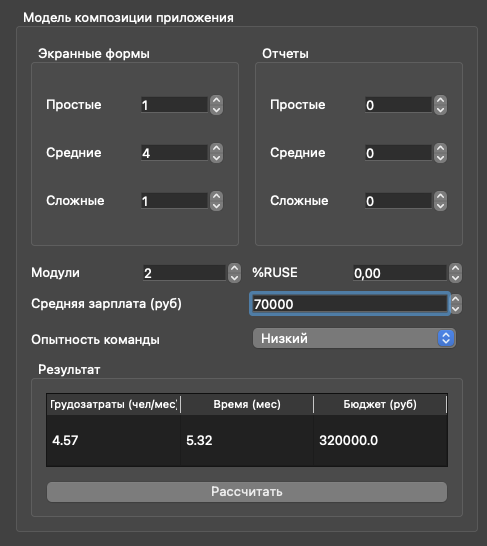
\includegraphics[scale=0.5]{inc/img/p_1.png}
	\end{center}
	\captionsetup{justification=centering}
	\label{fig:u3}
\end{figure}

Средняя численность команды определяется по следующей формуле:

$$\text{Численность команды} = \frac{\text{Трудозатраты}}{\text{Время}} =
\frac{4.57}{5.29} = 1 \text{ работник.}$$

Предварительная оценка бюджета для средней зарплаты 70 000 рублей проводится по
следующей формуле:

$$\text{Бюджет} = \text{Трудозатраты} \cdot \text{Средняя зарплата} = 4.57 \cdot
70 000 = 320 000\text{ рублей.}$$

%%%%%%%%%%%%%%%%%%%%%%%%%%%%%

\newpage

\subsection*{Метод функциональных точек}

\subsection*{Описание}

\textbf{Функциональная точка} --- это единица измерения функциональности программного
обеспечения.

\textbf{Пользователи} --- это отправители и целевые получатели данных, ими могут быть как реальные люди, так и смежные интегрированные информационные системы.

\textbf{Функциональные типы} — логических группы взаимосвязанных данных, используемых и поддерживаемых приложением:

\begin{itemize}
    \item[---] внешний ввод (EI) --- транзакция получения данных от пользователя;
    \item[---] внешний вывод (ЕО) ---  транзакция перечи данных пользователю;
    \item[---] внешний запрос (EQ) ---  интерактивный диалог с пользователем, требующий от него каких-либо действий и не связанный с вычислением производных данных или обновлением внутренних логических файлов (базы данных);
    \item[---] внутренний логический файл (ILF) --- информация, которая используется во внутренних взаимодействиях системы;
    \item[---] внешний интерфейсный файл (EIF) ---файлы, участвующие во внешних взаимодействиях с другими системами.
\end{itemize}

Для оценки сложности функциональных типов используются следующие характеристики (их количество):

\begin{itemize}
    \item[---] DET (data element type) --- это уникальное распознаваемое пользователем, неповторяющееся поле данных;
    \item[---] RET (record element type) --- идентифицируемая пользователем логическая группа данных внутри ILF или EIF;
    \item[---] FTR (file type referenced) --- это тип файла, на который ссылается транзакция.
\end{itemize}

Оценка числа функциональных точек происходит по алгоритму:

\begin{enumerate}
    \item определение функциональных типов приложения и их количества;
    \item определение количества связанных с каждым функциональным типом элементарных данных (DET), элементарных записей (RET) и файлов типа ссылок (FTR)
    \item оценка сложности каждого типа по соответствующим таблицам и определение количества функциональных типов каждой сложности;
    \item подсчет количества функциональных точек приложения, путем умножения числа количества функциональных типов каждой сложности на соответстсвующие коэффициенты и сложения полученных результатов;
    \item проведение корректировки числа функциональных точек  с учетом общих характеристик системы в соответствии с формулой:

    $$\text{AFP} = \text{FP} \cdot (0.65 + 0.01 \cdot \sum\limits_{i = 1}^{14} F_i),$$

    где $\text{FP}$ --- число функциональных точек, полученное на предыдущем шаге,

    $F_i$ --- $i$-ый коэффициент регулировки сложности, принимающий значения от 0~до~5~(нет влияния, случайное, небольшое, среднее, важное, основное), которое выбирается по соответствующей таблице.
\end{enumerate}

Из числа функциональных точек выводится количество строк кода по таблицам соответствия их числа (число строк кода на одну функциональную точку), построенных на основе статистических данных в зависимости от языка программирования.

\subsection*{Применение}

\subsubsection*{Постановка задачи}

Компания получила заказ на разработку клиентского мобильного приложения брокерской системы. Программа позволяет просматривать актуальную биржевую информацию, производить сделки и отслеживать их выполнение. Приложение имеет 4 страницы: авторизация, биржевые сводки, заявки, новая заявка.

\subsubsection*{Страница <<Авторизация>>}

На данной странице осуществляется ввод логина и пароля пользователя для входа в систему.
Страница содержит \textbf{два поля ввода} и \textbf{одну командную кнопку}, а также \textbf{флажок-переключатель}, который активируется при необходимости запоминания параметров авторизации.

По данной странице можно выделить следующий набор функциональных типов:

\begin{itemize}
    \item[---] внутренние логические файлы:
        \begin{itemize}
            \item[---] таблица пользователей бд с полями логина и пароля:

            $\text{DET} = 2$ --- логин, пароль;\\
            $\text{RET} = 1$ --- логин и пароль являются строками;\\
            Уровень:  низкий;
            
            \item[---] локальный файл для хранения данных одного пользователя:

            $\text{DET} = 2$ --- логин, пароль;\\
            $\text{RET} = 1$ --- логин и пароль являются строками;\\
            Уровень:  низкий;
            
        \end{itemize}
    \item[---] внешник логический файл: отсутствует;
    \item[---] внешний ввод: запоминание данных пользователя:
    
        $\text{DET} = 4$ --- логин, пароль, флажок, кнопка;\\
        $\text{FTR} = 1$ --- локальный файл для данных одного пользователя.\\
        Уровень: низкий;

    \item[---] внешний вывод: отсутствует;
    \item[---] внешний запрос: авторизация:

        $\text{DET} = 4$ --- логин, пароль, флажок, кнопка;\\
        $\text{FTR} = 1$ --- локальный файл для данных одного пользователя.\\
        Уровень: низкий.
\end{itemize}

Итого по странице:

\begin{itemize}
    \item[---] 2 ILF низкого уровня;
    \item[---] 1 EI низкого уровня;
    \item[---] 1 EQ низкого уровня.
\end{itemize}

\subsubsection*{Страница <<Биржевые сводки>>}

Страница содержит \textbf{таблицу}, \textbf{кнопку} «Добавить» и диалоговое окно с \textbf{одним полем для ввода} и \textbf{двумя командными кнопками}.

Таблица содержит три колонки: Ценная бумага (имя бумаги), Цена (цена за одну ценную бумагу), Изменение (изменение цены бумаги со времени последнего закрытия биржи). Кнопка «Добавить» вызывает \textbf{диалоговое окно} для добавления новой бумаги (окно состоит из поля ввода и кнопок ОК, Cancel).

По данной странице можно выделить следующий набор функциональных типов:

\begin{itemize}
    \item[---] внутренний логический файл: таблица ценных бумаг с полем имени:
    
        $\text{DET} = 1$ --- имя;\\
        $\text{RET} = 1$ --- имя --- строка;\\
        Уровень: низкий.
        
    \item[---] внешний логический файл: информация по цене и изменению о ценных бумагах;

        $\text{DET} = 3$ --- имя, цена, изменение;\\
        $\text{RET} = 1$ --- имя --- строка, цена и изменение --- вещественный тип;\\
        Уровень: низкий.
        
    \item[---] внешний ввод: добавление новой бумаги:
    
        $\text{DET} = 3$ --- текстовое поле для имени, кнопка <<Cancel>>, кнопка <<OK>>; \\
        $\text{FTR} = 1$ --- добавление записи во внутренний логический файл.\\
        Уровень: низкий.
        
    \item[---] внешний вывод информации по ценным бумагам:
    
        $\text{DET} = 3$ --- имя, цена, изменение; \\
        $\text{FTR} = 2$ --- обращение к внутреннему файлу с именами бумаг и к внешнему с информацией о цене и изменении;\\
        Уровень: низкий;
        
    \item[---] внешний запрос: отсутсвует.
\end{itemize}

Итого по странице:

\begin{itemize}
    \item[---] 1 ILF низкого уровня;
    \item[---] 1 EIF низкого уровня;
    \item[---] 1 EI низкого уровня;
    \item[---] 1 EO низкого уровня.
\end{itemize}

\subsubsection*{Страница <<Заявки>>}

Заявки содержат \textbf{таблицу}, отображающую текущие (еще не выполненные) заявки на покупку или продажу ценных бумаг. Таблица содержит четыре поля: Тип (покупка/продажа), Имя бумаги, Цена, по которой готовы покупаться/продаваться бумаги, Количество бумаг для покупки/продажи. При нажатии на любую строку таблицы появляется контекстное меню с возможностью \textbf{удалить} или \textbf{изменить заявку}.

По данной странице можно выделить следующий набор функциональных типов:

\begin{itemize}
    \item[---] внутренний логический файл: таблица текущих заявок:

        $\text{DET} = 4$ --- тип, имя, цена, количество;\\
        $\text{RET} = 4$ --- тип --- логический, имя --- строка, цена --- вещественное число; количество --- целое число;\\
        Уровень: низкий.
    
    \item[---] внешний логический файл: отсутствует
    \item[---] внешний ввод:
        \begin{itemize}
            \item удаление:
            
                $\text{DET} = 5$ --- тип, имя, цена, количество, кнопка; \\
                $\text{FTR} = 1$ --- обращение к внутреннему логическому файлу;\\
                Уровень: низкий;
                
            \item изменение:

                $\text{DET} = 5$ --- тип, имя, цена, количество, кнопка; \\
                $\text{FTR} = 1$ --- обращение к внутреннему логическому файлу;\\
                Уровень: низкий;
                
        \end{itemize}
    \item[---] внешний вывод информации о заявках:

        $\text{DET} = 4$ --- тип, имя, цена, количество; \\
        $\text{FTR} = 1$ --- обращение к внутреннему логическому файлу;\\
        Уровень: низкий;
    
    \item[---] внешний запрос: отсутсвует.
\end{itemize}

\begin{itemize}
    \item[---] 1 ILF низкого уровня;
    \item[---] 2 EI низкого уровня;
    \item[---] 1 EO низкого уровня.
\end{itemize}

\subsubsection{Страница <<Новая заявка>>}

Страница позволяет оформить заявку на покупку или продажу ценной бумаги. Страница состоит из \textbf{4 полей}: Бумага (имя бумаги), Цена (цена, по которой необходимо купить/продать бумагу), Покупка (булева переменная в значение true обозначает покупку, false – продажа) и кнопки «Оформить» - для подтверждения оформления заявки.

По данной странице можно выделить следующий набор функциональных типов:

\begin{itemize}
    \item[---] внутренний логический файл: тот же, что и на странице заявок;
    \item[---] внешний логический файл: отсутствует;
    \item[---] внешний ввод: создание новой заявки:

        $\text{DET} = 5$ --- поля ввода имя, цена, количество, флаг покупки и кнопка; \\
        $\text{FTR} = 1$ --- обращение к внутреннему логическому файлу;\\
        Уровень: низкий;
    
    \item[---] внешний вывод: отсутствует;
    \item[---] внешний запрос: отсутствует.
\end{itemize}

\begin{itemize}
    \item[---] 1 EI низкого уровня.
\end{itemize}

\subsubsection*{Расчеты}

Всего функциональных типов:

\begin{itemize}
    \item[---] 5 EI низкого уровня;
    \item[---] 2 EO низкого уровня;
    \item[---] 1 EQ низкого уровня;
    \item[---] 4 ILF низкого уровня;
    \item[---] 1 EIF низкого уровня.
\end{itemize}

Для уточнения числа функциональных точек используются следующие значения характеристики продукта:

\begin{itemize}
    \item[---] Обмен данными --- 5
    \item[---] Распределенная обработка --- 5
    \item[---] Производительность --- 3
    \item[---] Эксплуатационные ограничения по аппаратным ресурсам --- 2
    \item[---] Транзакционная нагрузка --- 3
    \item[---] Интенсивность взаимодействия с пользователем (оперативный ввод данных) --- 4
    \item[---] Эргономические характеристики, влияющие на эффективность работы конечных пользователей --- 1
    \item[---] Оперативное обновление --- 4
    \item[---] Сложность обработки --- 4
    \item[---] Повторное использование --- 0
    \item[---] Легкость инсталляции --- 1
    \item[---] Легкость эксплуатации/администрирования --- 2
    \item[---] Портируемость --- 2
    \item[---] Гибкость --- 2 
\end{itemize}

Результаты расчетов числа функциональных точек представлены на рисунке.

\begin{figure}[h!]
	\begin{center}
		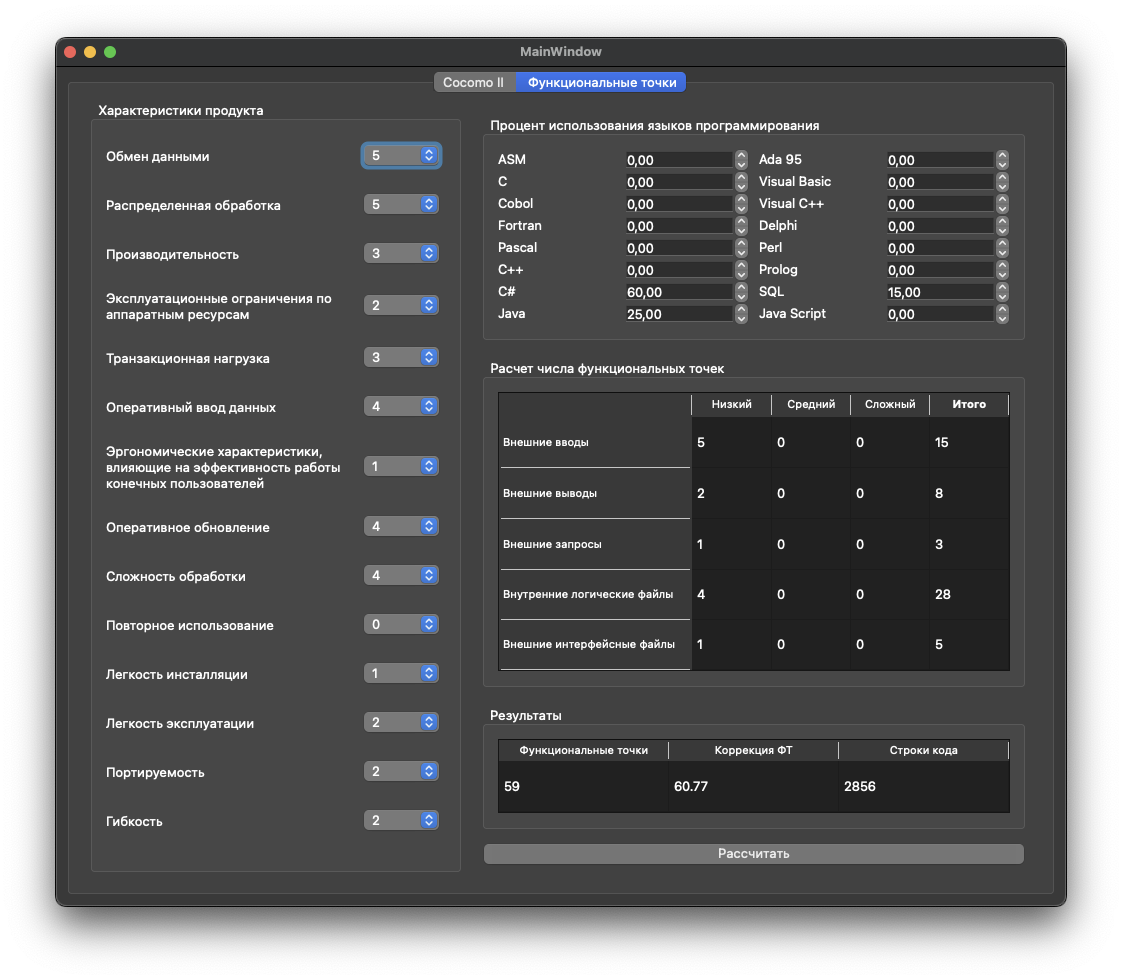
\includegraphics[scale=0.45]{inc/img/p_2.png}
	\end{center}
	\captionsetup{justification=centering}
	\label{fig:u3}
\end{figure}


Таким образом, число функциональных точек:

\begin{itemize}
    \item[---] первоначальное = 59;
    \item[---] скорректированное = 60.77.
\end{itemize}

Процентное соотношения языков программирования:

\begin{itemize}
    \item[---] SQL --- 15\%;
    \item[---] C\# --- 60\%;
    \item[---] Java --- 25\%.
\end{itemize}

С учетом данного соотношения с использованием таблиц соответствия числа функциональных точек строкам кода получаем, что проект будет состоять по данной оценке из 2856~строк кода.

%%%%%%%%%%%%%%%

\subsection*{Модель ранней разработки архитектуры в COCOMO=}

\subsubsection*{Описание модели}

Для получения приблизительных оценок проектных затрат периода выполнения проекта перед тем, как будет определена архитектура в целом, применяется модель ранней разработки архитектуры. Для такой модели характерны  оценки умеренной точности и ясно понимаемые особенности проекта, требования и архитектура. В качестве единиц измерения используются функциональные точки или KSLOC. 

Трудозатраты вычисляются так:

$$\text{Трудозатраты} = 2.45 \cdot \text{EArch} \cdot \text{Размер}^p,$$

\noindentгде $\text{Размер} = \text{KSLOC}$, $\text{EArch}$ определяется через произведение множителей трудоемкости:
$$\text{EArch} = \text{PERS} \cdot \text{RCPX} \cdot \text{RUSE} \cdot \text{PDIF} \cdot \text{PREX} \cdot \text{FCIL} \cdot \text{SCED}.$$

Время разработки получается в соответствии с формулой:

$$\text{Время} = 3 \cdot \text{Трудозатраты}^{0.33 + 0.2 \cdot (\text{p} - 1.01)},$$

\noindentгде $\text{p}$ --- показатель степени. Значение показателя степени рассчитывается с учетом факторов, влияющих на показатель степени:

$$\text{p} = \frac{(\text{PREC} + \text{FLEX} + \text{RESL} + \text{TEAM} + \text{PMAT})}{100} + 1.01.$$

\subsubsection*{Применение}

Из условия задания:

\begin{itemize}
    \item[---] надежность и сложность продукта (RCPX) --- очень высокие;
    \item[---]  повторное использование компонентов (RUSE) --- низкий;
    \item[---]  опытность персонала (PERS) --- низкая;
    \item[---]  способности персонала (PREX) --- номинальные;
    \item[---]  сложность платформы (PDIF) --- высокая;
    \item[---]  возможности среды (FCIL) --- очень высокие;
    \item[---]  сроки (SCED) --- очень высокие.
\end{itemize}

\subsubsection*{Результат}

На рисунке представлена оценка трудозатрат и длительности разработки с использованием модели ранней разработки архитектуры.

\begin{figure}[h!]
	\begin{center}
		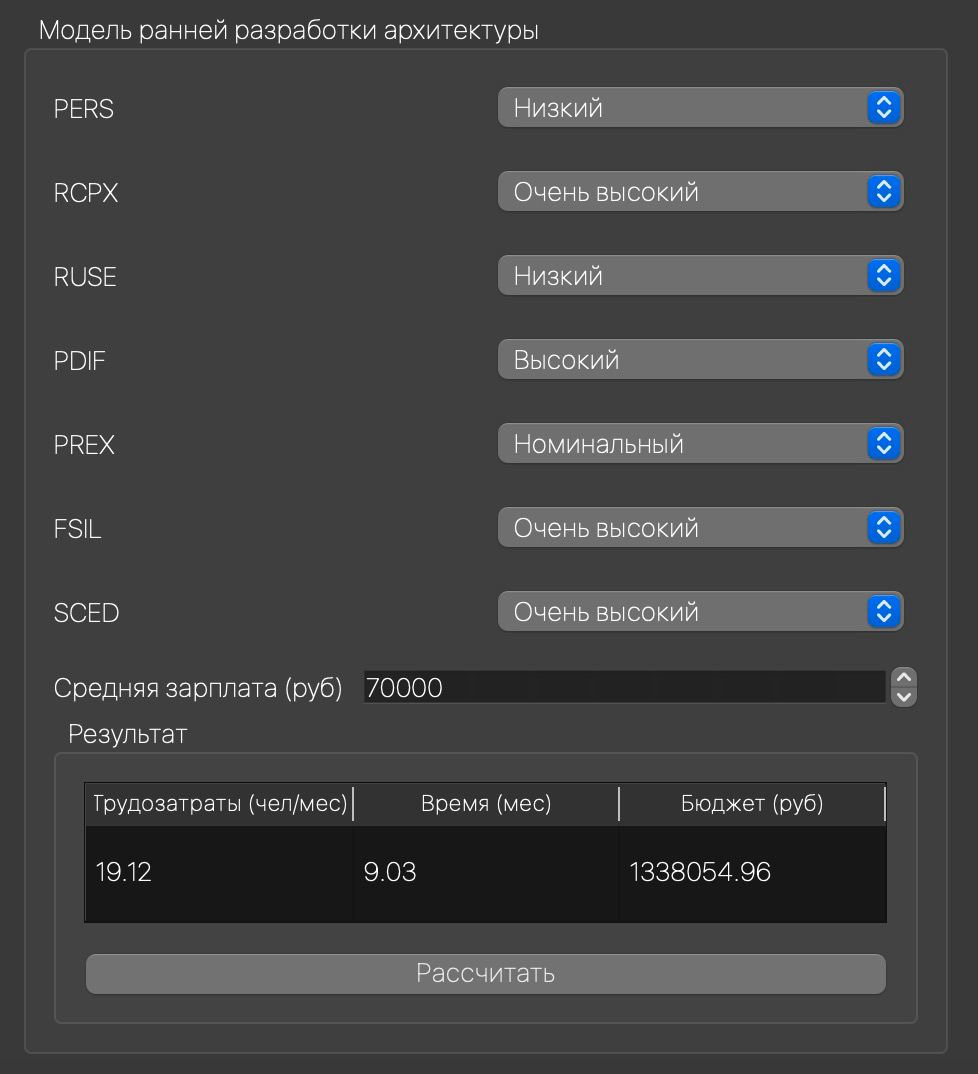
\includegraphics[scale=0.4]{inc/img/p_3.jpg}
	\end{center}
	\captionsetup{justification=centering}
	\label{fig:u3}
\end{figure}

Средняя численность команды определяется по следующей формуле:

$$\text{Численность команды} = \frac{\text{Трудозатраты}}{\text{Время}} = \frac{19.2}{9.03} = 3 \text{ работника.}$$

Предварительная оценка бюджета для средней зарплаты 70 000 рублей проводится по следующей формуле:

$$\text{Бюджет} = \text{Трудозатраты} \cdot \text{Средняя зарплата} = 19.12 \cdot 70 000 = 1 338 054.96 \text{ рублей.}$$

\subsection*{Вывод}

В ходе выполнения данной работы была освоена методология оценки
параметров проекта COCOMO2 и разработан программный инструмент для её
применения. Выполнен анализ выданного задания:

\begin{itemize}
    \item[---] рассчитаны функциональные точки и показатель степени модели (p);
    \item[---] были определены факторы, влияющие на показатель степени;
    \item[---] рассчитаны трудозатраты и времени по моделям ранней разработки архитектуры приложения и композиции приложения.
\end{itemize}

По модели композиции приложения прогноз более благоприятный, чем в
модели ранней архитектуры приложения.

Методология COCOMO2 является более сложной по сравнению с COCOMO,
но позволяет более тонко настраивать параметры плана, что даёт более точный
и детальный прогноз.